\documentclass[a4paper, 12pt]{article}

\usepackage[no-math]{fontspec-xetex}
\setmainfont{CMU Serif}
\usepackage[english, russian]{babel}

\usepackage{blindtext}
\usepackage{microtype}
\usepackage{geometry}

\usepackage{amsmath, amsfonts, amssymb, amsthm, mathtools}
\usepackage{MnSymbol}
\usepackage{physics}

\usepackage{graphicx, wrapfig, caption, subcaption}
\usepackage{color, xcolor}

\usepackage{hyperref}

\graphicspath{{figures/}}
\geometry{margin=6em}
\geometry{bottom=6em}

\hypersetup{colorlinks=true, linkcolor=blue, urlcolor=blue}

\title{Затухающие колебания в RLC контуре}
\author{Николай Грузинов}
\date{22 января 2021}

\begin{document}
\maketitle

Поскольку работа предполагала следование методичке, буду краток.
\begin{center}
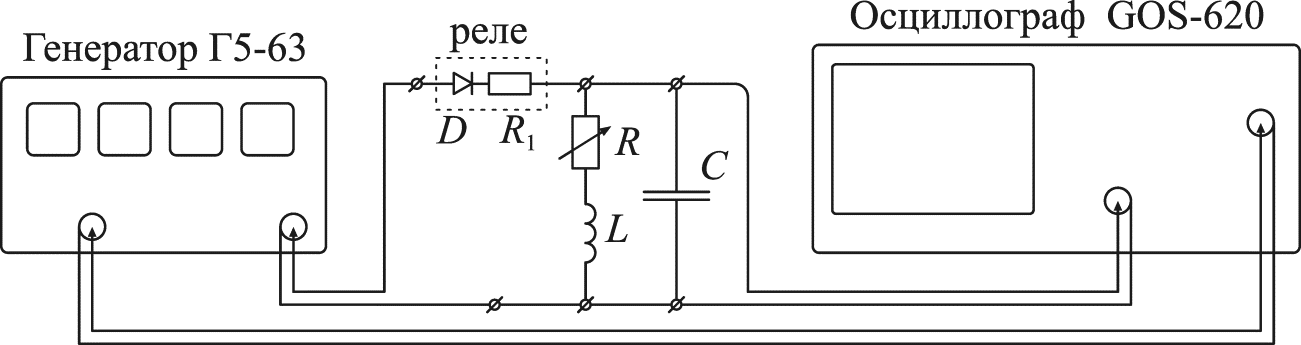
\includegraphics[width=0.7\linewidth]{curcuit.png}
\end{center}

\section{Задачи}
\begin{enumerate}
\item измерить периоды колебаний при нулевом сопротивлении реостата, проверить формулу $T = 2 \pi \sqrt{LC}$
\item выбрав конкретный конденсатор, подобрать с помощью реостата критическое сопротивление для данного контура
\item для этого конденсатора измерить добротность / декремент затухания колебаний для разных сопротивлений с помощью амплитуд на пиках затухающей синусоиды
\item то же самое, только в XY-режиме осциллографа.
\item по зависимости декремента затухания от сопротивления реостата вычислить критическое сопротивление контура, сравнить с подобранным экспериментально.
%\item измерив сопротивление и индуктивность катушки, прикинуть добротность контура по формуле $Q = \frac{1}{R} \sqrt{\frac{L}{C}}$
%\item сравнить значения добротности, полученные разными способами, проанализировать возможные расхождения
\end{enumerate}

\section{Результаты}
Значения емкостей конденсаторов измерены в методичке правильно, я проверил.
Катушку использовал на 400 витков.

\begin{tabular}{|c|c|}        \hline
ёмкость, нФ & период, мкс  \\ \hline
21.86       & 77           \\ \hline
33.23       & 92           \\ \hline
50.72       & 110          \\ \hline
70.83       & 130          \\ \hline
100.3       & 160          \\ \hline
223.6       & 240          \\ \hline
477.5       & 340          \\ \hline
927.7       & 480          \\ \hline
\end{tabular}

\begin{center}
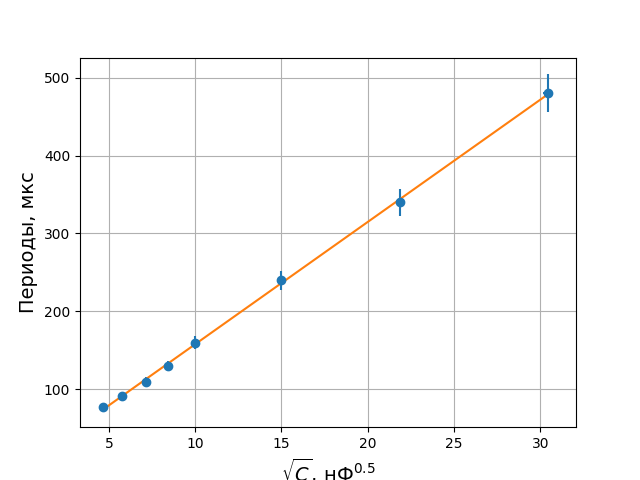
\includegraphics[width=0.5\linewidth]{check_periods.png}
\end{center}

Для дальнейших измерений выбрал пятый конденсатор, потому что для конденсаторов с меньшей емкостью нельзя было подобрать критическое сопротивление (сопротивления реостата не хватало), а поскольку в дальнейшем нужны были доли критического сопротивления, то хотелось, чтобы оно составляло большую часть от сопротивления реостата, и конденсаторы с большей емкостью не подходили.

Далее $C =$~100.3~нФ.
Характеристическая частота для 400-витковой катушки и этого конденсатора: $\frac{1}{T} =$~6.4~кГц.
Индуктивность и сопротивление катушки при маленьких частотах: 5.841~мГн, 3.5~Ом.
На частоте 10 кГц: 6.139~мГн, 8.3 Ом.
На характеристической частоте: 5.97~мГн, 6.7~Ом.

Критическое сопротивление \emph{реостата} для данного контура: $440 \pm 10$~Ом при полном сопротивлении реостата 466 Ом.
Погрешность оценил по чувствительности пика на картинке осциллографа к изменениям --- при меньших изменениях не видел разницы.

Измерение амплитуд по пикам для сопротивления реостата 23, 34, 44, 55 и 65~Ом:
\begin{table}[h]
23~Ом~\begin{tabular}{|c|c|}
\hline
Номер пика & Амплитуда, дел. \\ \hline
1 & 7.9 \\ \hline
2 & 5.5 \\ \hline
3 & 3.8 \\ \hline
4 & 2.6 \\ \hline
5 & 1.8 \\ \hline
\end{tabular}

34~Ом~\begin{tabular}{|c|c|}
\hline
Номер пика & Амплитуда, дел. \\ \hline
1 & 9.75 \\ \hline
2 & 5.9 \\ \hline
3 & 3.6 \\ \hline
4 & 2.2 \\ \hline
5 & 1.4 \\ \hline
\end{tabular}

44~Ом~\begin{tabular}{|c|c|}
\hline
Номер пика & Амплитуда, дел. \\ \hline
1 & 8.2 \\ \hline
2 & 4.4 \\ \hline
3 & 2.4 \\ \hline
4 & 1.3 \\ \hline
5 & 0.7 \\ \hline
\end{tabular}

55~Ом~\begin{tabular}{|c|c|}
\hline
Номер пика & Амплитуда, дел. \\ \hline
1 & 7.0 \\ \hline
2 & 3.25 \\ \hline
3 & 1.4 \\ \hline
4 & 0.65 \\ \hline
\end{tabular}

65~Ом~\begin{tabular}{|c|c|}
\hline
Номер пика & Амплитуда, дел. \\ \hline
1 & 11.6 \\ \hline
2 & 4.8 \\ \hline
3 & 1.9 \\ \hline
4 & 0.75 \\ \hline
\end{tabular}

\end{table}
\begin{center}
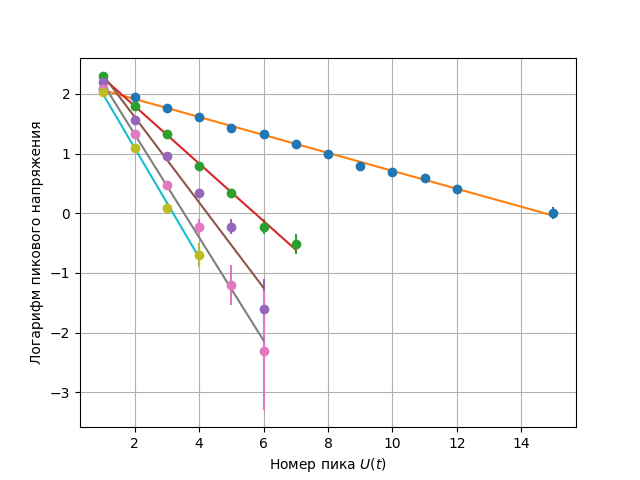
\includegraphics[width=0.7\linewidth]{qfactor_peaks.png}
\end{center}

Измерение амплитуд по спирали:

\begin{tabular}{|c|c|c|c|c|}
\hline
Номер пика & Амплитуда при 23 Ом, дел. & При 34 Ом & При 44 Ом & При 55 Ом \\ \hline
1 & 9    & 10.4 & 8.2 & 7.6  \\ \hline
2 & 6.6  & 7.0  & 4.7 & 3.7  \\ \hline
3 & 4.8  & 4.5  & 2.6 & 1.7  \\ \hline
4 & 3.4  & 2.8  & 1.4 & 0.8  \\ \hline
5 & 2.4  & 1.8  &     &      \\ \hline       
6 & 1.6  &      &     &      \\ \hline      
\end{tabular}
\begin{center}
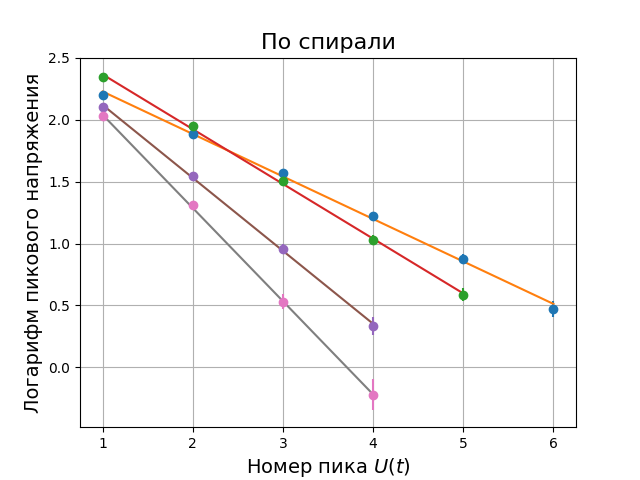
\includegraphics[width=0.7\linewidth]{qfactor_peaks_spiral.png}
\end{center}

Из графиков можно достать зависимость углового коэффициента $-\Theta$ (декремент затухания) от сопротивления реостата $r$.
Теоретически, должно получаться $\Theta = \frac{2 \pi r}{R_{\text{cr}}}$.
По наклону прямой на графике можно определить, что $R_{\text{cr}} = 467$~Ом.

\begin{center}
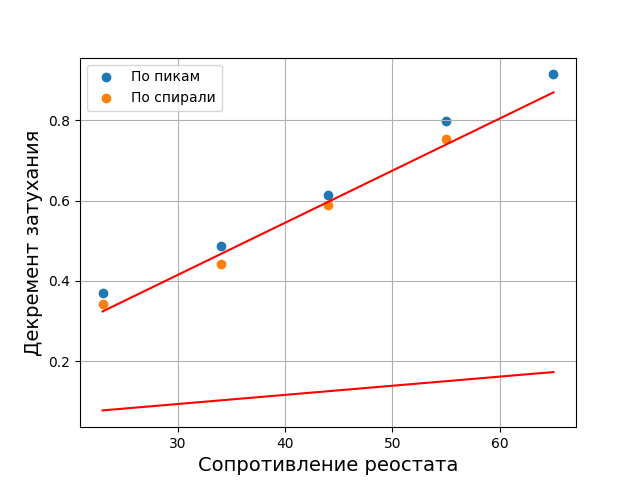
\includegraphics[width=0.7\linewidth]{qfactor_prop_r.png}
\end{center}

\section{Выводы}

Все, что должно было лечь на прямую, легло.

Критическое сопротивление $R_{\text{cr}} = 467$~Ом, полученное из графика $\Theta(r)$, существенно отличается от того, что я ожидал: критическое сопротивление реостата 440$\pm$10~Ом + примерно 7~Ом на сопротивление катушки.
Скорее всего, я где-то ошибся, либо недооцениваю погрешность измерения декремента затухания.

График $\Theta(r)$ выглядит подозрительно из-за того, что все желтые точки (измерение по спирали) ниже синих.
Возможно, когда я измерял добротность по пикам, я забыл убрать постоянное смещение напряжения, из-за чего образовалась маленькая систематическая ошибка.

Для вывода о погрешности добротности мне стоило набрать больше точек (я ограничивался пятью), однако это оказалось муторно из-за необходимости переключать масштаб осциллографа (это неудобно, потому что приходится в уме переводить всё в вольты).

\end{document}
